% !TEX root = ../main.tex
\documentclass[../main.tex]{subfiles}
\begin{document}

\section{Mathematical description of the poly-line separation measure}
\label{appendix:clustering_maths}

This appendix details the metric used in Section \ref{sec:aggregation_of_volunteer_models} to cluster poly\-lines used by volunteers to model spirals arms. It can be seen as a variant of the Fréchet distance. The metric is illustrated in Figure \ref{fig:spiral_metric_description}.

\begin{figure}
  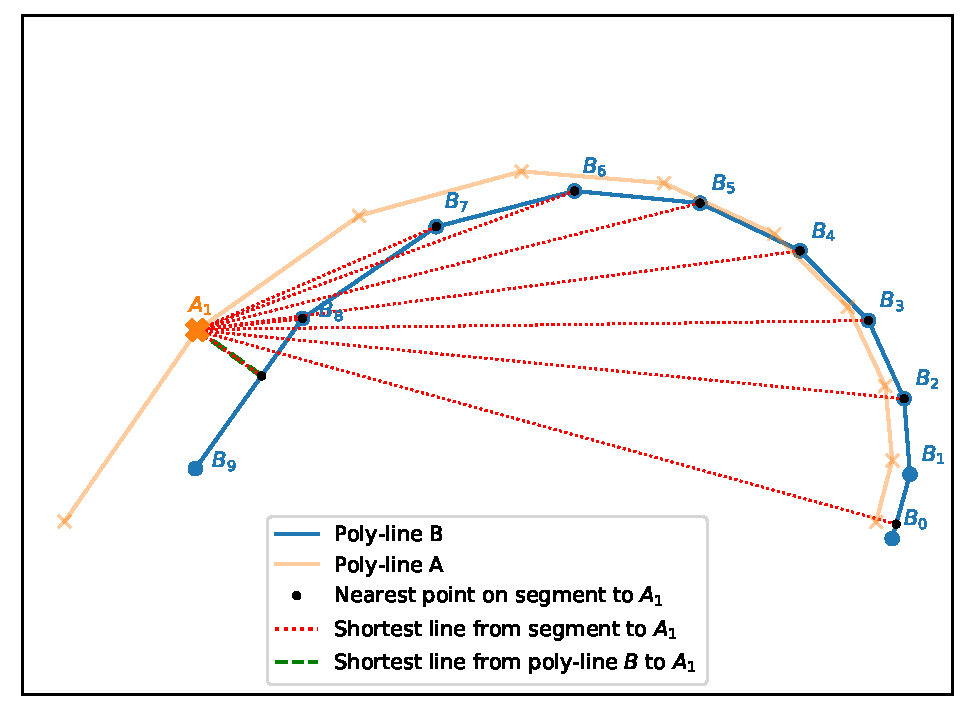
\includegraphics[width=8cm]{images__appendix/spiral_metric_description.pdf}
  \caption{Illustration of the metric used. For each point in line $A$, the shortest distance to each segment in line $B$ is calculated (shown as dotted red lines). The minimum of these distances (corresponding to the line shown in dashed green) is squared.}
  \label{fig:spiral_metric_description}
\end{figure}

First, define a poly-line containing $n$ 2D cartesian coordinates (vertices) as

\begin{equation}
A: \{i \in \mathbb{N};\;i<n\} \longrightarrow \mathbb{R}
^2\end{equation}

We also define a function, $t$, which calculates how far a point $\vec{p}$ is along the line between two other points ($\vec{v}$ and $\vec{w}$):

\begin{equation}
t(\vec{p},\,\vec{v},\,\vec{w}) \equiv \frac{(\vec{p} - \vec{v})\cdot(\vec{v} - \vec{w})}{|\vec{w} - \vec{v}|^2}.
\end{equation}

The minimum distance from $\vec{p}$ to the line segment between $\vec{v}$ and $\vec{w}$ is given by

\begin{equation}
d(\vec{p},\,\vec{v},\,\vec{w}) = \|\left(\vec{v} + \mathrm{min}(\mathrm{max}(t(\vec{p},\,\vec{v},\,\vec{w}),\, 0),\, 1)\;(\vec{w} - \vec{v})\right) - \vec{p}\|
\end{equation}

We then define a ``squared distance'' from the poly-line $A$ (containing $n$ vertices) to the poly-line $B$ (containing $m$ vertices):

\begin{equation}
D(A,\,B) \equiv \frac{1}{n}\sum_{i = 0}^{n} \mathrm{min}\{j \in \mathbb{N}_0,\, j < m;\; d(A_i,\, B_j,\, B_{j+1})^2\}.
\end{equation}

The choice to square the distances and penalize large deviations from other lines was a data-driven choice to improve the results of clustering.

Finally, we define our separation measure between two drawn poly-lines as

\begin{equation}
distance(A,\,B) \equiv D(A,\,B) + D(B,\,A).
\end{equation}


\section{Ancillary Tables}
\begin{table*}
  \centering
  \caption{The maximum, minimum and default values for model parameters. Note that some parameters were allowed to overflow when fitting, for instance an axis ratio greater 1 (signifying a swap of major and minor axis) was allowed, and corrected for once fitting reached completion. This helped avoid the optimizer encountering parameter bounds and failing to converge. Component roll was similarly unconstrained.}
  \begin{tabular}{l|l|r|r|r|r|r}
\hline
Component & Parameter &  Default &  Volunteer allowed &  Volunteer allowed & Tuning Minimum & Tuning Maximum \\
 &  &   &  Minimum &  Maximum & Bound & Bound \\
\hline
disc   & axRatio &      0.5 &       0.0 &      inf &       0.01   & 100   \\
       & scale   &      2.0 &       0.0 &     1.00 &       0      & inf   \\
       & i0      &      1.0 &       0.0 &     0.20 &       0      & inf   \\
bulge  & axRatio &      0.5 &       0.0 &      inf &       0.01   & 100   \\
       & scale   &      2.0 &       0.0 &     1.00 &       0      & inf   \\
       & i0      &      2.0 &       0.0 &     0.50 &       0      & inf   \\
       & n       &      5.0 &       0.5 &     1.00 &       0.1    & 10    \\
bar    & roll    &      0.0 &      -inf &      inf &       0.01   & 100   \\
       & scale   &      2.0 &       0.0 &     1.00 &       0      & inf   \\
       & i0      &      1.0 &       0.0 &     0.20 &       0      & inf   \\
       & n       &      2.0 &       0.3 &     0.50 &       0.1    & 10    \\
       & c       &      3.0 &       1.5 &     2.00 &       0.01   & 10    \\
spiral & i0      &      1.0 &       0.0 &     0.75 &       0      & inf   \\
       & spread  &      2.0 &       0.0 &     1.00 &       0      & inf   \\
       & falloff &      2.0 &       0.0 &     1.00 &       0.01   & inf   \\
\hline
  \centering
  \end{tabular}
  \label{table:bad_values}
\end{table*}

\begin{table*}
  \centering
  \caption{Pivot table of reported errors on parameters for our sample of 297 galaxies. All errors apart from $b/a$ are relative errors.}
  \begin{tabular}{l|l|rrrrrrrr}
  \hline
  component & parameter &  count &  mean &   std &   min &   25\% &   50\% &   75\% &    max \\
  \hline
  disc  & $b/a$      &  292 &  0.09 &  0.04 &  0.01 &  0.06 &  0.09 &  0.12 &  0.20 \\
        & $\Sigma_e$ &  292 &  0.51 &  0.25 &  0.06 &  0.30 &  0.47 &  0.69 &  1.20 \\
        & $r_e$      &  292 &  0.18 &  0.05 &  0.04 &  0.14 &  0.17 &  0.21 &  0.34 \\
  bulge & $b/a$      &  273 &  0.10 &  0.05 &  0.00 &  0.07 &  0.10 &  0.14 &  0.23 \\
        & $\Sigma_e$ &  273 &  0.50 &  0.25 &  0.00 &  0.32 &  0.51 &  0.68 &  1.31 \\
        & $n$        &  273 &  0.69 &  0.27 &  0.00 &  0.47 &  0.76 &  0.90 &  1.26 \\
        & $r_e$      &  273 &  0.15 &  0.07 &  0.00 &  0.10 &  0.14 &  0.19 &  0.44 \\
  bar   & $b/a$      &   81 &  0.07 &  0.03 &  0.01 &  0.05 &  0.07 &  0.09 &  0.14 \\
        & $c$        &   81 &  0.13 &  0.08 &  0.00 &  0.08 &  0.13 &  0.20 &  0.35 \\
        & $\Sigma_e$ &   81 &  0.56 &  0.37 &  0.00 &  0.23 &  0.53 &  0.87 &  1.37 \\
        & $n$        &   81 &  0.47 &  0.30 &  0.00 &  0.22 &  0.51 &  0.73 &  0.97 \\
        & $r_e$      &   81 &  0.18 &  0.09 &  0.02 &  0.13 &  0.17 &  0.23 &  0.44 \\
  \hline
  \end{tabular}
  \label{table:error_values}
\end{table*}
\end{document}
